\section{Appendix}\label{ap:appendix}

\subsection{Bayesian PK Model Details}

The Bayesian model used to predict personalized concentration in response to dose, which we refer to as $ \mathcal{M}_1 $, is 

\begin{align}\label{model_M1}
	y_{i,j} &\sim \Lognormal  \left(  C_i(t_j)  , \sigma^2_y \right)  \\
	\sigma^2 &\sim \Lognormal \left( 0.1, 0.2 \right)\\	
	C_i(t_j) &= \begin{dcases}
	\frac{D_{i} \cdot F}{C l_{i}} \cdot \frac{k_{e, i} \cdot k_{a, i}}{k_{e, i}-k_{a, i}}\left(e^{-k_{a, i}\left(t_{j}-\delta_{i}\right)}-e^{-k_{e, i}\left(t_{j}-\delta_{i}\right)}\right) & t_j>\delta_i \\
	0 & \mbox{else}
	\end{dcases}\\
	k_{e,i} &= \alpha_i \cdot k_{a,i}\\
	k_{a,i} &= \dfrac{\log(\alpha_i)}{t_{max, i}\cdot(\alpha_i-1)}\\
	\delta_i &\sim \operatorname{Beta}(\phi, \kappa) \\
	\operatorname{logit}(\alpha_i) \vert \beta_\alpha, \sigma^2_\alpha &\sim \Normal(\mu_\alpha + \mathbf{x}_i^T \beta_\alpha, \sigma^2_\alpha)\\
	\log(t_{max, i}) \vert \beta_{t_{max}}, \sigma_{t_{max}} &\sim \Normal(\mu_{t_{max}} + \mathbf{x}^T_i \beta_{t_{max}}, \sigma^2_{t_{max}}) \\
	\log(Cl_i) \vert \beta_{Cl}, \sigma_{Cl} &\sim \Normal(\mu_{Cl} + \mathbf{x}^T_i \beta_{Cl}, \sigma^2_{Cl}) \\ \nonumber \\
	p(\phi) &\sim \operatorname{Beta}(20, 20)\\
	p(\kappa) &\sim \operatorname{Beta}(20, 20)\\
	p(\mu_{Cl}) &\sim \Normal(\log(3.3), 0.15^2)\\
	p(\mu_{t_{max}}) &\sim \Normal(\log(3.3), 0.1^2)\\
	p(\mu_{\alpha}) &\sim \Normal(-0.25, 0.5^2)\\
	p(\sigma_y) &\sim \Lognormal(\log(0.1), 0.2^2)\\
	p(\sigma_{CL}) &\sim \Gmma(15, 100)\\
	p(\sigma_{t_{max}}) &\sim \Gmma(5, 100)\\
	p(\sigma_{\alpha}) &\sim \Gmma(10, 100)\\
	p(\beta_{Cl, k}) &\sim \Normal(0, 0.25^2) \quad k = 1 ...	 4\\
	p(\beta_{t_{max}, k}) &\sim \Normal(0, 0.25^2) \quad k = 1 ... 4\\	
	p(\beta_{\alpha, k}) &\sim \Normal(0, 0.25^2) \quad k = 1 ... 4
\end{align}

Here, normal distributions are parameterized by their mean and variance, lognormal distributions are parameterized by the mean and variance of the random variable on the log scale, and gamma distributions are parameterized by their shape and rate.  The $\mu$ in the model above represent population means on either the log or logit scale, the $\beta$ are regression coefficients for the indicated pharmacokinetic parameter, the sigmas are the population level standard deviations on the log or logit scale, $\delta$ is aparameter which relaxes the assumption that the dose is absorbed into the blood immeditately upon ingestion, $F$ is the bioavailability of apixiban (which we fix to 0.5 \cite{byon2019apixaban}) and $D$ is the size of the dose in milligrams.  All continuous variables were standardized using the sample mean and standard deviation prior to being passed to the model. 



\begin{table}\label{tab:coefs}
	\centering
	\begin{tabular}[t]{rccc}
		\toprule
		& $\beta_\alpha$ & $\beta_{Cl}$ & $\beta_{t_{max}}$\\
		\midrule
		\cellcolor{gray!6}{Age} & \cellcolor{gray!6}{-0.08 (-0.27,0.1)} & \cellcolor{gray!6}{0.01 (-0.06,0.08)} & \cellcolor{gray!6}{-0.01 (-0.1,0.08)}\\
		Creatinine & -0.06 (-0.25,0.14) & 0.02 (-0.05,0.09) & -0.05 (-0.14,0.04)\\
		\cellcolor{gray!6}{Sex} & \cellcolor{gray!6}{-0.2 (-0.53,0.15)} & \cellcolor{gray!6}{0.39 (0.23,0.54)} & \cellcolor{gray!6}{-0.01 (-0.18,0.15)}\\
		Weight & 0.32 (0.11,0.55) & 0.2 (0.12,0.27) & 0.09 (0.01,0.18)\\
		\bottomrule
	\end{tabular}
	\caption{Posterior means for coefficients for each covariate in our pharmacokinetic model.  In parantheses are 95\% credible interval estimates.}
\end{table}


Once fit, $ \mathcal{M}_1$ can be used to predict the pharmacokinetics of new patients, using the patient’s covariates as predictors.  To do so, the marginal posterior distributions for $ \mu_{Cl} $, $ \mu_{t_{max}} $, $ \mu_{\alpha}$, $ \beta_{Cl} $, $ \beta_{t_{max}} $, $ \beta_{\alpha} $, $ \sigma_{Cl} $, $ \sigma_{t_{max}} $, $ \sigma_{\alpha} $, and $ \sigma_y $ must be summarized.  We use maximum likelihood on the posterior samples to summarize the marginal posterior distributions. We model the population means  and regression coefficients as normal, and the standard deviations  as gamma.  The maximum likelihood estimates are used to construct priors for a new model, which we call $ \mathcal{M}_2 $. We construct $ \mathcal{M}_2 $ so as to be able to predict plasma concentration after multiple doses (of potentially different sizes) administered over time, and remove the time delay ($ \delta $) to simplify our simulations.  Model priors for $ \mathcal{M}_2 $ are then 

\begin{align}
	p(\mu_{Cl}) & \sim \Normal(0.5, 0.04) \\
	p(\mu_{t_{max}}) & \sim \Normal(0.93, 0.05) \\
	p(\mu_\alpha) &\sim \Normal(-1.35, 0.13)\\
									\nonumber \\
	p(\sigma_{Cl}) &\sim \Gmma(69.15, 338.31)\\
	p(\sigma_{t_{max}}) &\sim \Gmma(74.96, 349.56)\\
	p(\sigma_{\alpha}) &\sim \Gmma(10.1, 102.07)\\
									\nonumber\\
	p(\beta_{Cl, 1}) &\sim \Normal(0.39, 0.08^2)\\
	p(\beta_{Cl, 2}) &\sim \Normal(0.19,0.04^2)\\
	p(\beta_{Cl, 3}) &\sim \Normal(0.02,0.04^2)\\
	p(\beta_{Cl, 4}) &\sim \Normal(0.01,0.04^2)\\
									\nonumber\\
	p(\beta_{t_{max}, 1}) &\sim \Normal(-0.01, 0.08^2)\\
	p(\beta_{t_{max}, 2}) &\sim \Normal(0.09,0.05^2)\\
	p(\beta_{t_{max}, 3}) &\sim \Normal(-0.05,0.04^2)\\
	p(\beta_{t_{max}, 4}) &\sim \Normal(-0.01,0.04^2)\\
										\nonumber\\
	p(\beta_{\alpha, 1}) &\sim \Normal(-0.19, 0.17^2)\\
	p(\beta_{\alpha, 2}) &\sim \Normal(0.33,0.11^2)\\
	p(\beta_{\alpha, 3}) &\sim \Normal(-0.06,0.1^2)\\
	p(\beta_{\alpha, 4}) &\sim \Normal(-0.09,0.1^2)\\
\end{align}

For our experiments, we generate the pharmacokinetic parameters of 1000 simulated patients from the prior predictive model of $ \mathcal{M}_2 $. Bayesian models are generative models, meaning they can generate pseudodata by drawing random variables according to the model specification going from top (model priors) to bottom (model likelihood).  To do so, we begin by resampling 1000 tuples of age, sex, weight, and creatinine from the dataset used to fit $ \mathcal{M_1} $. We sample one draw of r $ \mu_{Cl} $, $ \mu_{t_{max}} $, $ \mu_{\alpha}$, $ \beta_{Cl} $, $ \beta_{t_{max}} $, and $ \beta_{\alpha} $  from their respective prior distributions in  $ \mathcal{M}_2 $. The values of these parameters remained fixed for all 1000 patients. Conditioned on the values of these mus and betas, we compute the expectation of the population distribution for each pharmacokinetic parameter by computing $ \mu_{Cl} + \mathbf{x}^T \beta_{Cl} $, $ \mu_{t_{\max}} + \mathbf{x}^T \beta_{t_{max}} $,  $ \mu_{\alpha} + \mathbf{x}^T \beta_{\alpha} $, where $\mathbf{x}^T$ is the resampled tuple.  From the prior distribution of M2, we sample one draw of$ \sigma_{Cl} $, $ \sigma_{t_{max}} $, $ \sigma_{\alpha} $, and $ \sigma_y $.  These remained fixed for all 1000 patients. Using the previously computed expectations and $\sigma$, we sample 1000 tuples of pharmacokinetic parameters, one for each of the simulated patients.  The clearance rate and time to max concentration were sampled assuming a lognormal distribution.  Alpha was sampled using a logitnormal distribution. The pharmacokinetics can then be determined conditional on the pharmacokinetic parameters. Each of simulated patients' pharmacokinetic parameters remained fixed through the experiments.  We simulate the latent concentration using $ C(t) $ as written in $\mathcal{M}_2$, and can simulate observed concentrations by drawing a sample from a lognormal distribution with mean $\ln(C(t))$ and standard deviation $ \sigma_y$

We use Stan, an open source probabilistic programming language, for fitting our Bayesian models via Hamiltonian Monte Carlo (a Markov Chain Monte Carlo technique) and computing markov chain diagnostics. Twelve chains are initialized and run for 2000 iterations each (1000 for warmup allowing the Markov chain the opportunity to find the correct target distribution and 1000 to use as samples from the posterior).


\subsection{Diagnostics For Bayesian Models Fit Via MCMC}

Once the form of the model is specified, creating simulated patients or estimating the PK parameters of a real patient requires computation of or sampling from the posterior distribution of the relevant variables given the relevant data. However, exact computation of the posterior distribution is intractable for all but very simple models, so Markov chain Monte Carlo (MCMC) techniques are often used to approximate the expectations with respect to the posterior distribution.  Presently, the gold standard for generating samples from the posterior is Hamiltonian Monte Carlo (HMC), which works by generating a sequence of samples that ``explores'' the posterior distribution by solving a system of ordinary differential equations which describe the motion of an imaginary particle as it rolls along the surface of the log posterior density.  Many implementations of HMC come with diagnostics which monitor the behaviour of the Markov chains that are used to generate samples and help to ensure that they are representative of the posterior distribution. That these Markov chains behave well is crucial, as any inferences about or from the model are obtained from samples generated by the chains. To assess the quality of the Markov chains, several diagnostics are commonly used including: number of divergences, the Gelman-Rubin convergence diagnostic, and effective sample size \cite{betancourt2018conceptual}.

In practice, several Markov chains are used simultaneously to generate samples from the posterior. The chains are assessed with within-chain and between-chain diagnostics. First, individual chains may sometimes \textit{diverge}. A divergence in a Markov chain indicates that the HMC Markov chain has encountered a region of high curvature in the posterior distribution which cannot be adequately explored.  Consequently, Monte Carlo estimators of any expectations can be biased due to incomplete exploration of the posterior distribution.  It is important that none of the Markov chains generated by HMC display a divergence, and that many chains (typically 4 or more) are initialized and are allowed to explore the posterior distribution. 

Having ensured that no chains are diverging, a group-level diagnostic is used to assess whether all chains have converged to the same limiting distribution.  The \textit{Gelman-Rubin (sometimes called $\hat{R}$) convergence diagnostic} is designed to detect if the Markov chains have converged to the same distribution by measuring the within-chain variance to the between chain-variance. In practice, $1.05<\hat{R}$ indicates that there is poor mixing of the Markov chains and inference from the samples should not be performed lest the Monte Carlo estimators are biased by this poor mixing.

Even if the chains do not exhibit divergences and arrive at the same limiting distribution, the Markov chains could still exhibit high within-chain correlation, thereby increasing the uncertainty of estimation of key posterior quantities such as means, variances, or quantiles \cite{brooks2011handbook}.  The \textit{effective sample size} is a measure of how much the within chain autocorrelation increases uncertainty estimates.  Presently, the guidance is that the effective sample size ratio should be larger than $100 \times (\mbox{number of chains})$ \cite{vehtari2019rank}.

In addition to monitoring divergences, Gelman-Rubin convergence diagnostics, and effective sample sizes, the model should be evaluated against existing domain knowledge.  Evaluating that the model has learned appropriate  behaviour (e.g. that as one quantity increases, another should decrease) can be performed by plotting model predictions.  Additionally, \textit{posterior predictive checks} -- generating synthetic data  from the model's posterior distribution and comparing against the real data -- can be performed to ensure the model is not generating data which are physically impossible or completely unrealistic. Once the model is fit, important diagnostics indicate no pathological behaviour, and the model is deemed to fit the data sufficiently well, the model can then used to generate synthetic pharmacokinetic data for use in experiments to compare different forms of personalization. Each generated data point may be thought of as one synthetic patient, with observed covariates and observed pharmacokinetic parameters. These parameters, which are never observed in real data, allow us to compute the effects of any dosing decisions (which are made \textit{without} direct knowledge of the parameters), and thus allow us to evaluate the performance of different modes of personalized dosing on the sampled population. 

\section{Bayesian Model Diagnostics for Case Study}

\begin{figure}
	\centering
	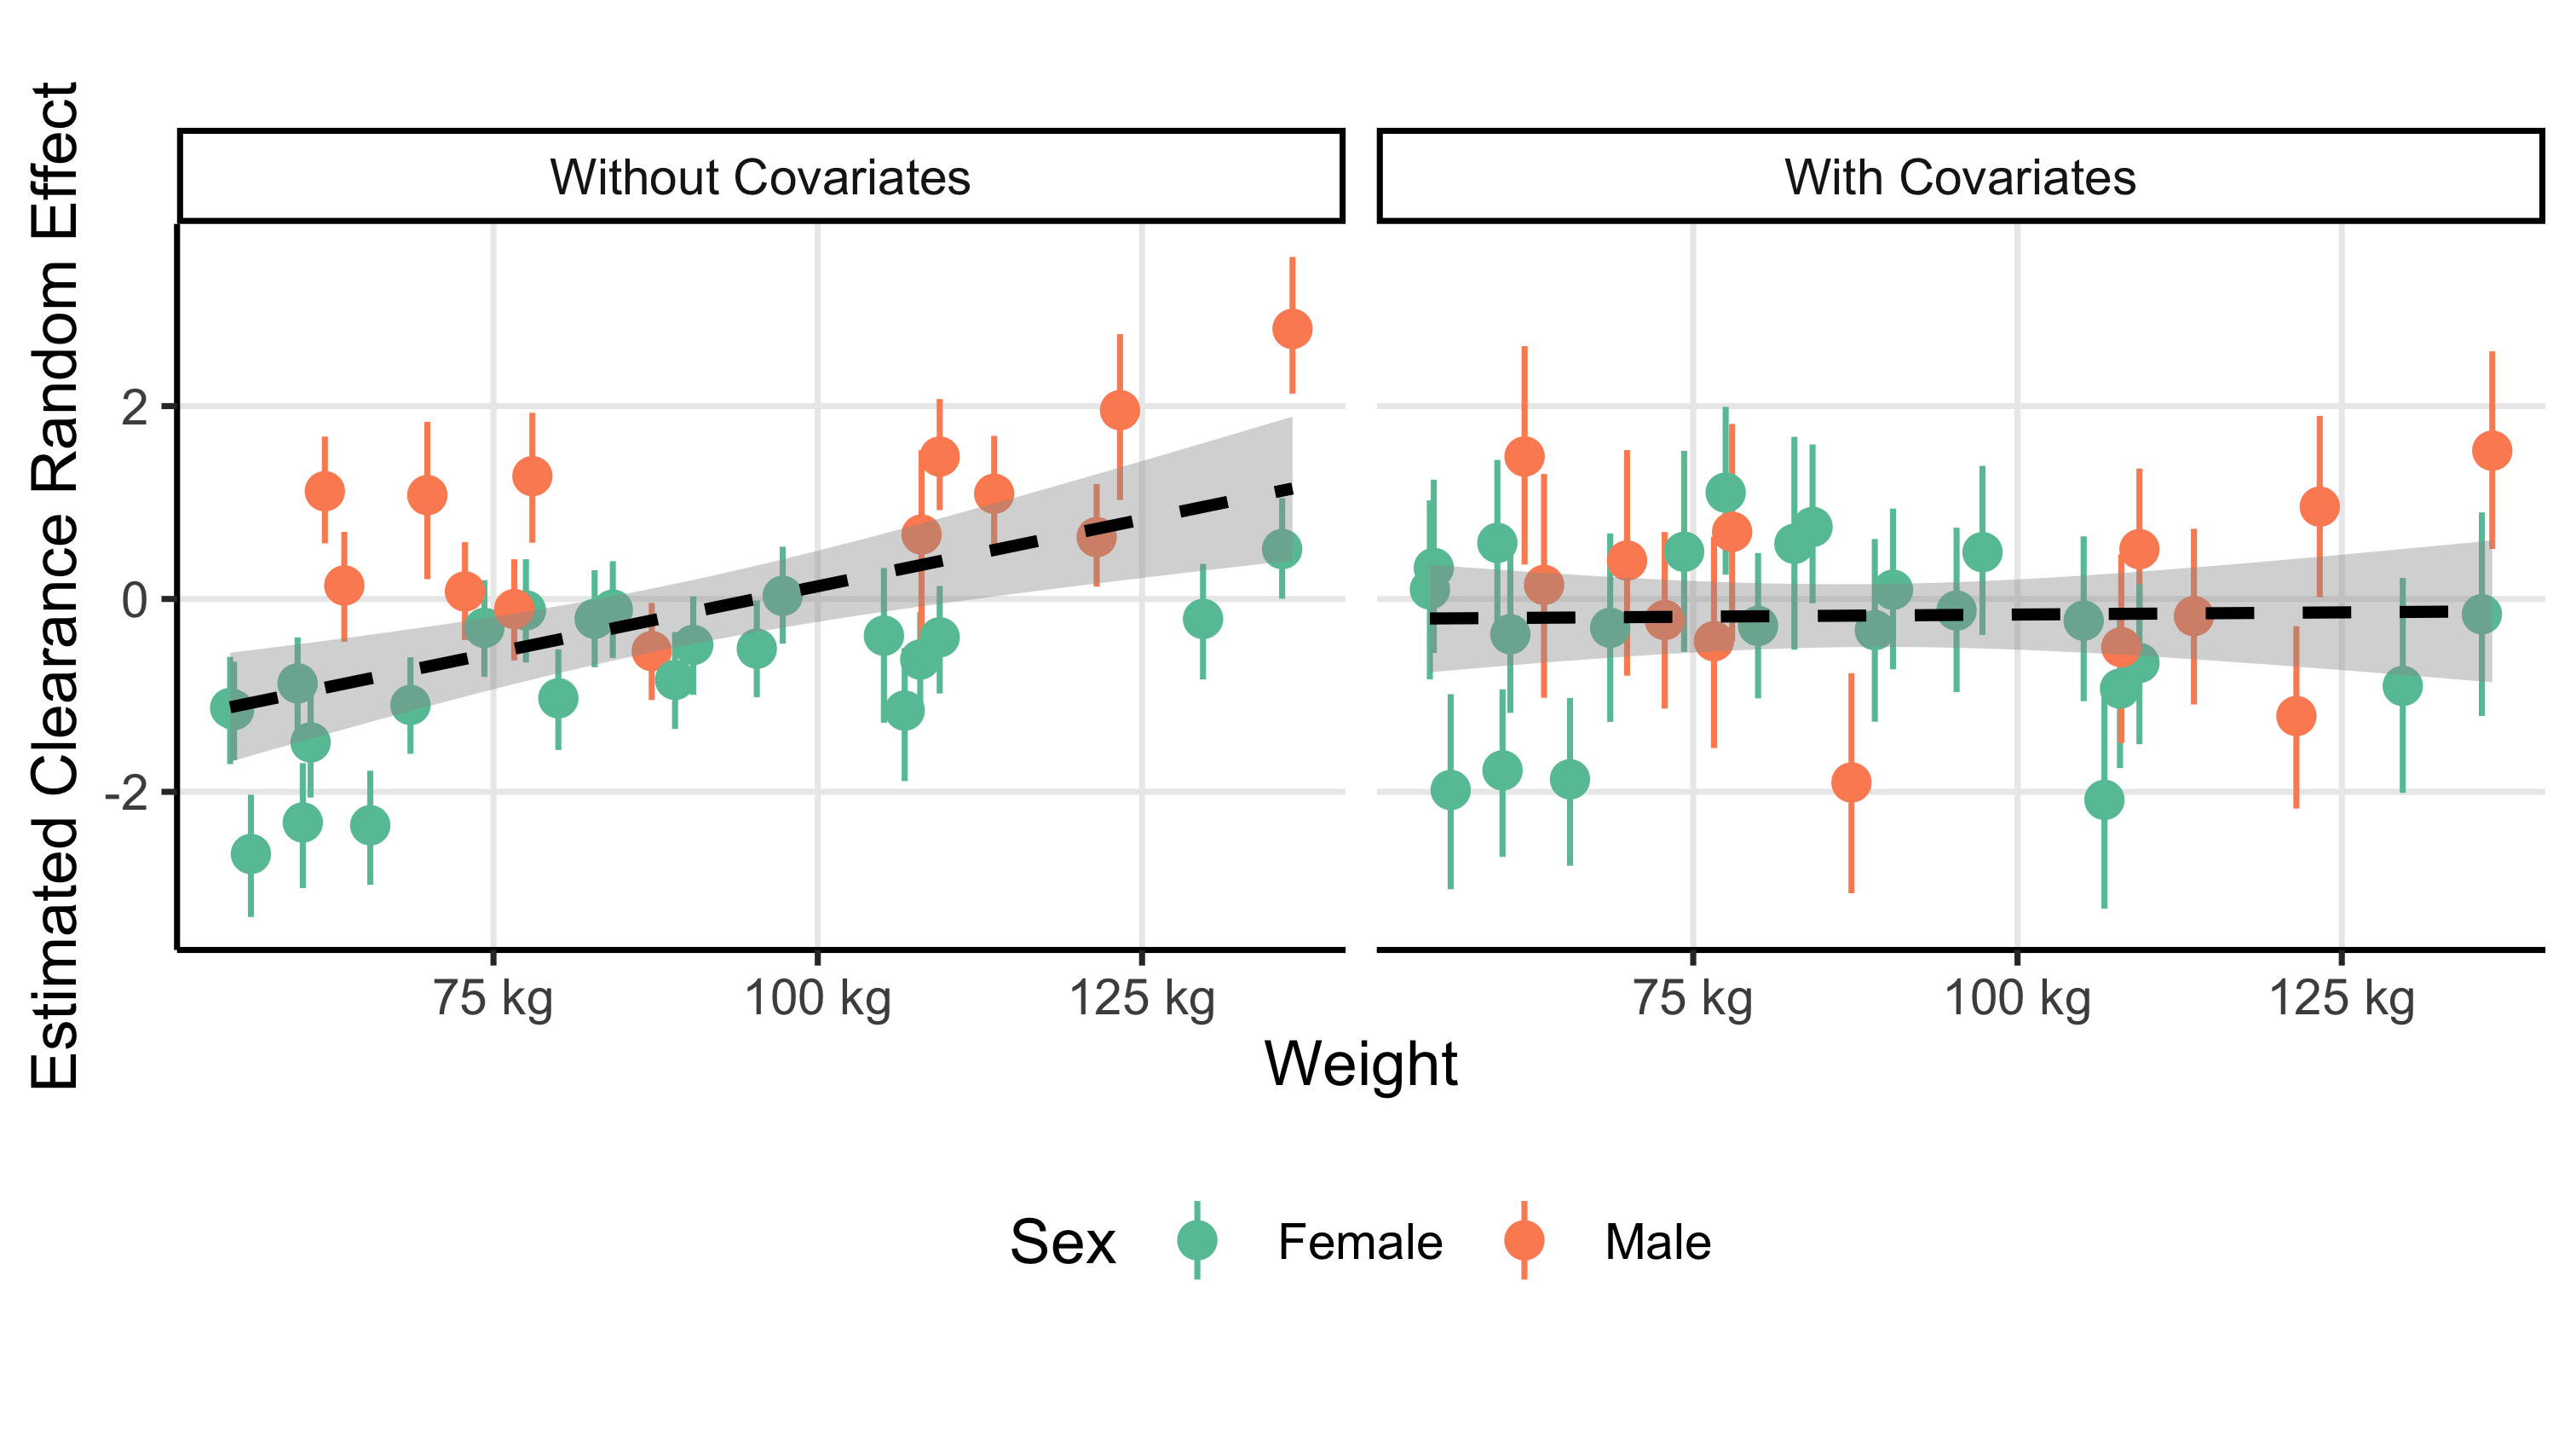
\includegraphics[width=\linewidth]{"figures/random_effects_change.png"}
	\caption{Random effects estimates for clearance $ CL_i $ and 95\% credible intervals (left).  Random effects estimates are colored by patient sex.  Prior to adjusting for covariates, a general trend in weight can be seen in the random effects.  Patients who are heavier tend to have larger random effect, and males tend to have larger random effects than females of the same weight.  Patterns such as these indicate that weight and sex can be used to explain variation in the random effects.  After adjusting for sex and weight (right), the random effects have no discernable pattern.}
	\label{fig:randomeffectschange}
\end{figure}

We fit our model to real pharmacokinetic data using the open source probabalistic programming language, Stan \cite{gelman2015stan}.  Stan monitors several Markov chain diagnostics, none of which detected problematic Markov chain behavior, which indicates that Stan’s sampling algorithm was able to converge (0 divergences, all all Gelman-Rubin diagnostics<1.01, all effective sample sizes  > 2600).  

The inclusion of covariates in the model results in a better fit than excluding them. Shown in \cref{fig:randomeffectschange} are the estimated random effects for the clearance pharmacokinetic parameter of each patient as a function of weight.  Patient sex is indicated by color, the overall trend is shown in the black dashed line.  Failing to include patient sex and weight results in males having on average a larger random effect than females of the same weight, and heavier patients having a larger random effect than lighter patients.  When covariates are added into the model, the variation in the random effects attenuates, resulting in closer alignment to model assumptions. A better fit to the data means data generated from the model may be closer aligned with the true data generating process.

Examining the posterior distributions of the regression coefficients provides further insights into the relationships between covariates and pharmacokinetics. Greater patient weight is associated with an increase in the expected value of alpha (which is used to compute the elimination and absorption rates in the first order one compartment PK model.  The parameter $ \alpha $ is the ratio of how fast the drug exits the central compartment  how fast the drug enters the central compartment) which impacts the time to maximum concentration after each dose.  There is an estimated effect of sex on $ \alpha $ (males have smaller alpha than females, meaning the drug leaves their central compartment slower or enters the central compartment quicker), however the uncertainty is large (estimated effect -0.2 on the logit scale, 95\% credible interval -0.53 to 0.15). See \cref{tab:coefs} in the Appendix for a full summary of the regression coefficients.


%\begin{figure}
%	\centering
%	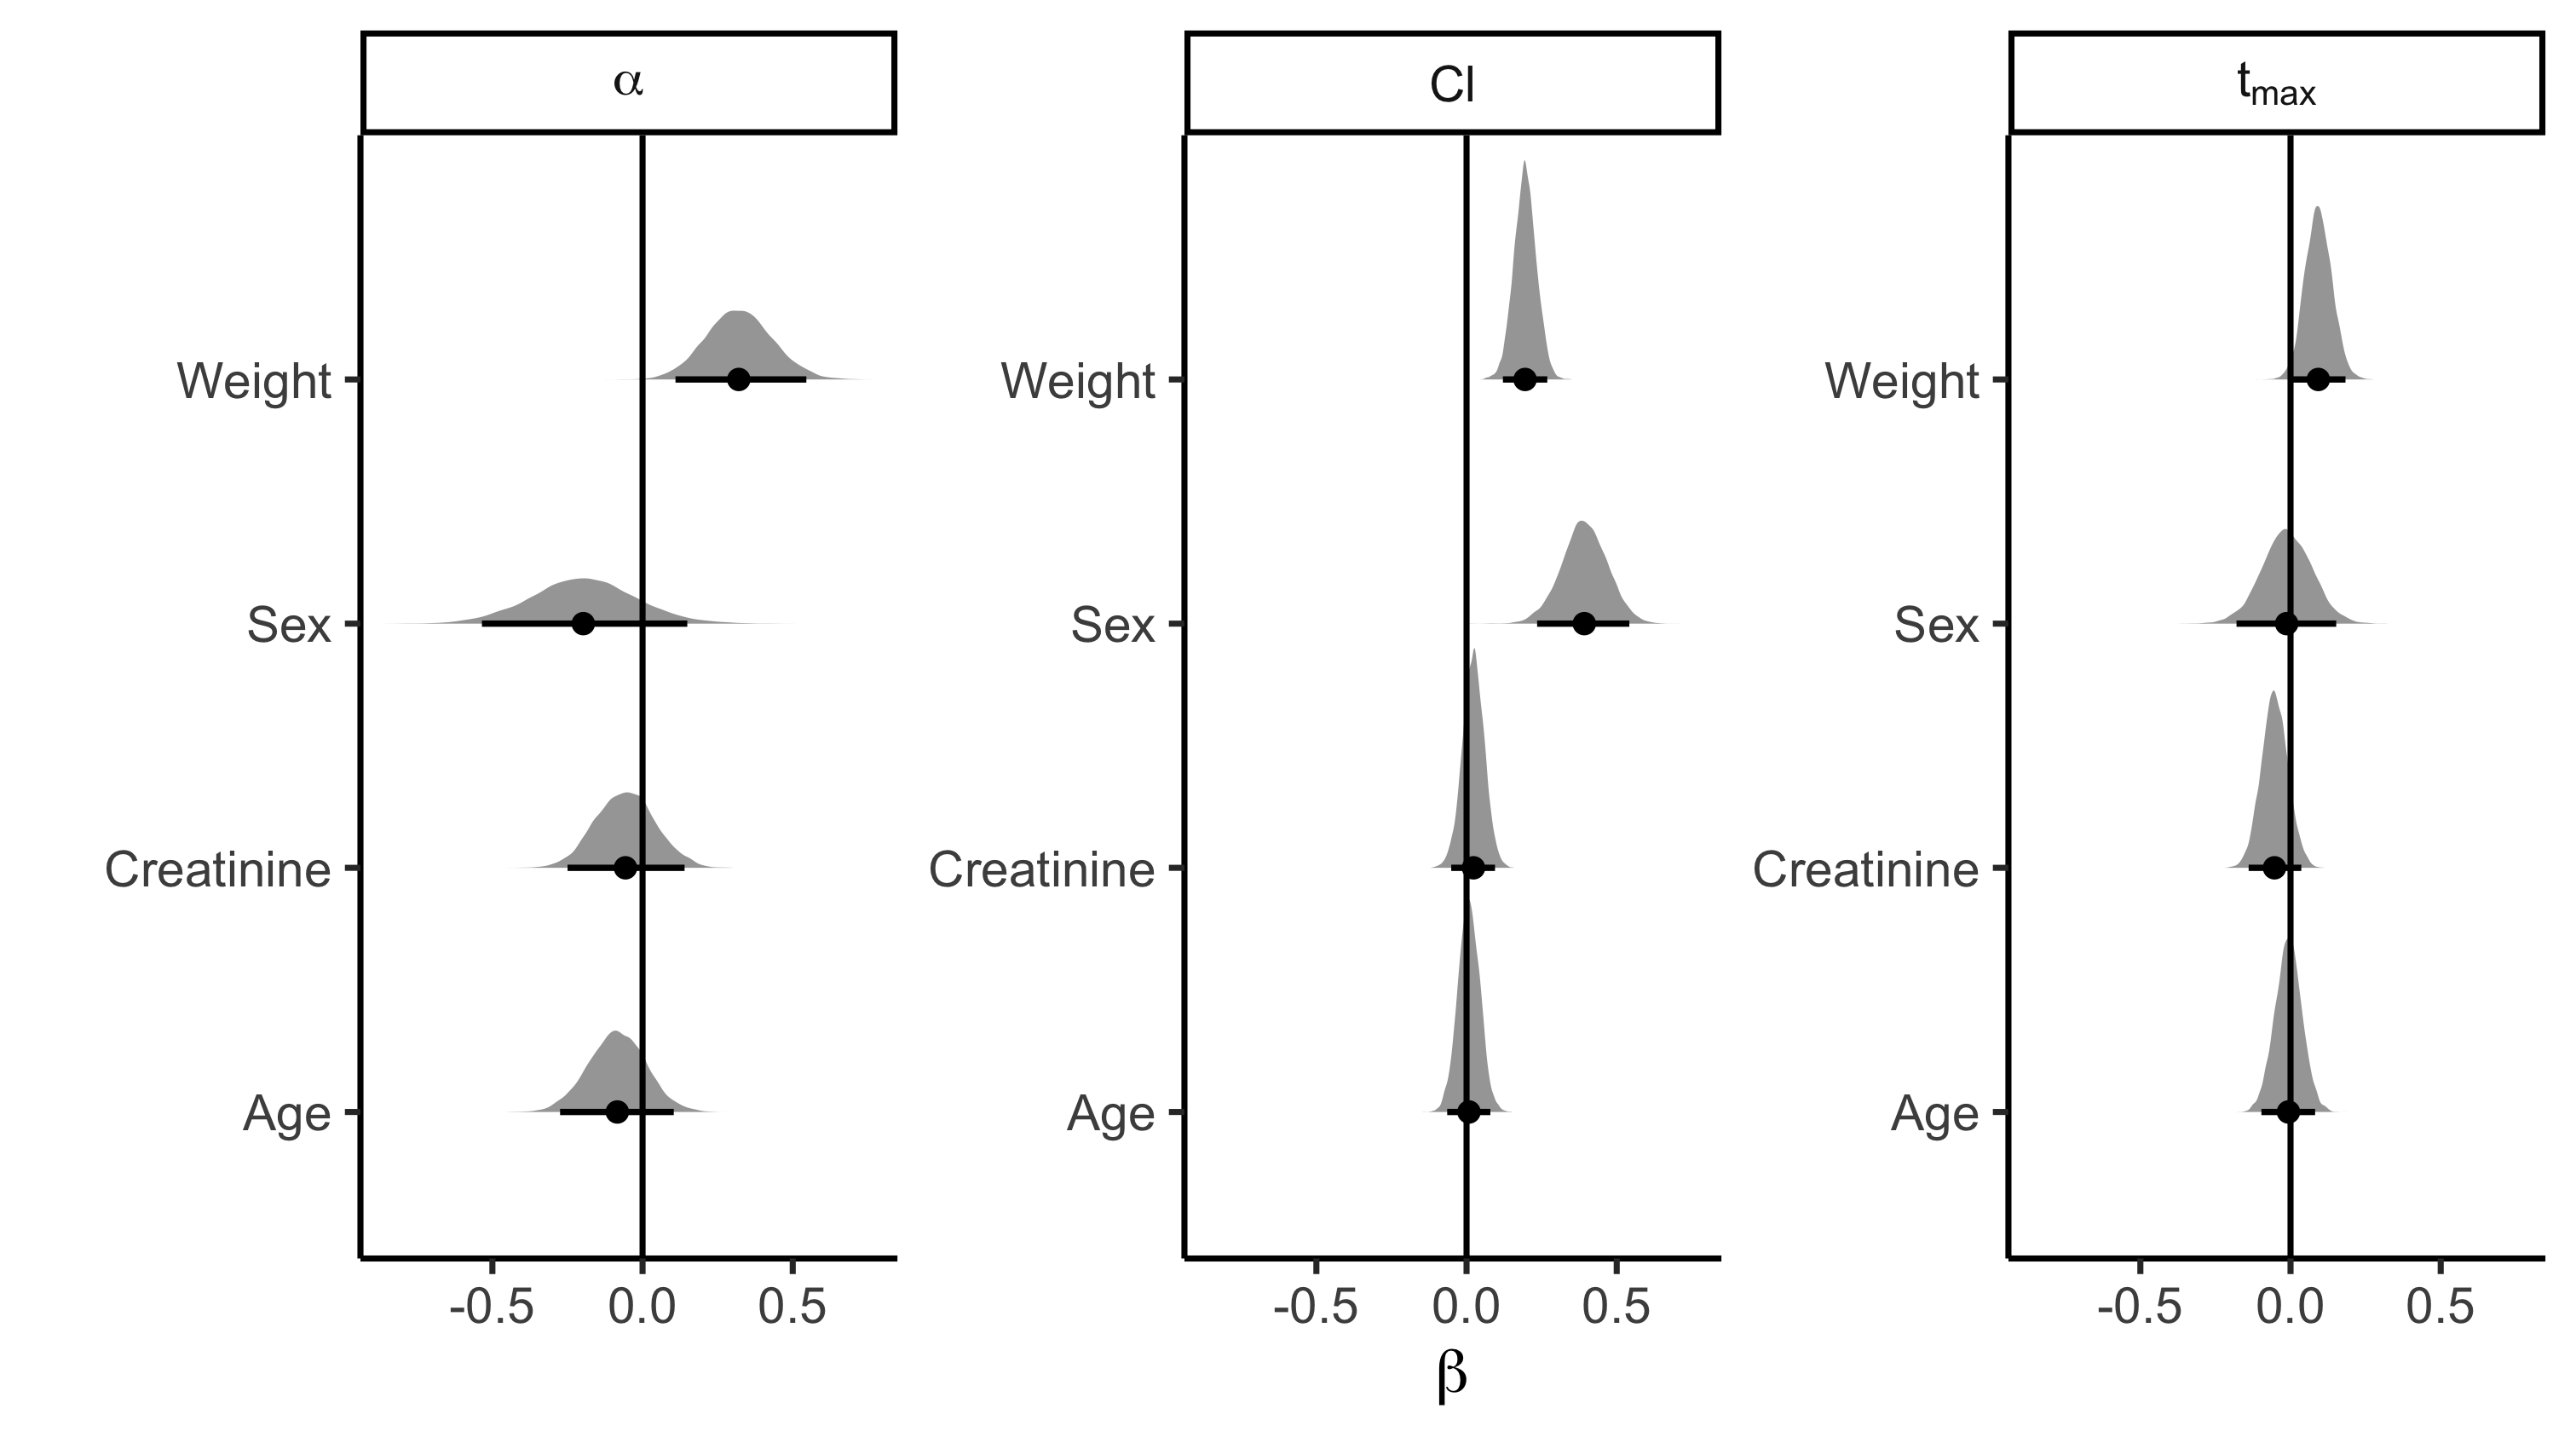
\includegraphics[width=1\linewidth]{figures/coef_vals}
%	\caption{Posterior distributions of regression coefficients. Expectations are shown as black dots, 95\% credible intervals are shown as horizontal black lines.  Solid black vertical line is $\beta=0$ for reference.  Note, regression coefficients for $Cl$ and $t_{max}$ act multiplicatively (a one unit increase in weight leads to a change in $Cl$ of $\exp(\beta)$), while regression coefficients for $\alpha$ are interpreted on the log odds scale.}
%	\label{fig:coefvals}
%\end{figure}


Model training error is comparable between the two models; the model without covariates achieves an average error of 8.31 ng/ml as measured by root mean squared error.  The model with covariates achieves a root mean squared error of 8.36  ng/ml.  Estimates of concentration uncertainty remain similar between the two models as well.  We conclude the inclusion of covariates in the model improves model inferences but does not substantially improve the fit of the model in this case.

While prediction error and concentration uncertainty are comparable between the two models, the most important differences are between inter-individual uncertainty.  The inclusion of the covariates explains variation between individual pharmacokinetic parameters, hence the between patient variability $\sigma_{Cl}, \sigma_{t_{max}}$ and $\sigma_\alpha$ are smaller in the covariate model as opposed to the no covariate model.  This uncertainty effects decision making, as the no covariate model is more uncertain about the pharmacokinetics of new patients.